\chapter{Developing common representations in AI and humans}
\label{chap:common_representations}

In this Chapter we study how human representation and AI representation can be combined, and how brain data can be infused into neural networks.

\section[Using human brain activity to guide machine learning]{\textit{Using human brain activity to guide machine learning}\\ \mandatory{fong2017using}}

This study tries to \textbf{improve ML performance by guiding it with brain activity}, and explore whether such guidance makes the representations themselves more ``human-like". Notice that here the focus is not on performance but on \textbf{representational geometry}. The underlying idea is that, if the human brain is a natural reference point (for representation geometry) and performance, and ANNs are a good algorithm for learning structure, then we can attempt to leverage the ML algorithm with biological information.\\

They consider 7 brain areas (ROIs, \textit{regions of interest}, whose partitioning is defined a-priori). Different brain areas code for different information about the stimulus, but all of them are involved in \textbf{visual processing} (either low, middle, or high level). They use two types of models: CNN and HOG (\textit{histogram of oriented gradients}, an often-used algorithm for generating features that capture the local ``slopeness" of different parts of an image).

Their idea is to train a classifier on brain data to perform binary classification. To do so (to maximize the margin between the decision boundary and the data points), they use a loss derived from the \textbf{Hinge loss} \notet. They define the \textbf{``response strength" from brain fMRI activity data} as the \textbf{distance of an object from the decision boundary} for a given binary classification task.
This produces a per-stimulus activity weight (response strength) for each stimulus. As input to the classifier, each image is encoded as a vector of brain activity values sampled from a given brain area (one of the 7 mentioned before).
From the Hinge loss they define the \textbf{Activation weighted loss} (AWL) as:
\[
\phi (x, z) = max(0, (1-z) \cdot M(x,z)
\]
where $M(x,z) =\begin{cases}
         1+c_x, \text{if } z<1\\
        1 \text{ otherwise}
        \end{cases}$

and $c_x \geq 0$ is an activity weight derived from fMRI data corresponding to $x$ (it is the distance of the object from the classification boundary of the binary classifier trained on brain data).\\
While HL penalizes misclassified examples, \textbf{AWS penalizes misclassified examples on stimuli that are easy for humans to distinguish}.\\

They train a classifier on brain responses (fMRI), then use this prior knowledge to train a new model on non-annotated data. They basically use the learned weights as a starting point. The process consists in the following steps:
\begin{enumerate}
    \item \textbf{Derive per-stimulus ``activity weigths" from fMRI data}:
        \begin{itemize}
        \item collect \textit{per-stimulus} activity vectors: use fMRI to record bold response of subject;
        \item train a classifier on fMRI activity vectors: SVM classifier trained and tested;
        \item activity weights derived from distance boundary: use transformed classification scores.
    \end{itemize}
    \item \textbf{Train (calibrate) 2 image classifiers}:
    \begin{itemize}
        \item Conventional image classifier training: Radial Basis Function SVM classifier;
        \item Margins reweighted by activity data: SVM classifier with activity weighted loss function (note that not all training samples require fMRI weight).
    \end{itemize}
\end{enumerate}

They use images from 5 categories, and the classification problems are based on CNN or HOG features. Information from the higher-level cortical regions is combined in all possible combinations to produce feature sets.

\boxc{\notet Hinge loss}{
The true label is denoted as $t$ ($t=1$ or $t=-1$), while $y$ is the predicted activation for an object by the classifier. $t \cdot y$ is therefore the distance from the boundary. The Hinge loss wants to push this distance so that the margin from the boundary is above 1: 
\[
Loss(y) = max(0, 1-ty)
\]
if $ty <0$ (i.e., incorrect classification) $\Rightarrow 1-ty > 1$;\\
if $0< ty <1$ (correct classification but below the margin) $\Rightarrow 1-ty>0$;\\
if $ty>1$ (correct classification above the margin) $\Rightarrow  1-ty < 0$.\\
This means that the HL is proportional to the distance from the decision boundary, and it \textbf{does not care about magnitude of correct decisions above the margin}.\\

However, in \cite{fong2017using} they use a different formulation:
\[
\phi_h(z) = max(0,1-z)
\]
where $z = y \cdot f(x)$, $y \in N$ is the true label, and $f(x) \in \mathbb{R}$ is the predicted output; thus, $z$ denotes the correctness of a prediction. The HL function assigns a penalty to all misclassified data that is proportional to how erroneous the prediction is.
}

\subsection{Results}
They argue that brain activity compensates for poor feature representation (consider the large difference for HOG in Figure \ref{fig:fong}).

\begin{figure}[!ht]
    \centering
    \captionsetup{width=.8\linewidth}
    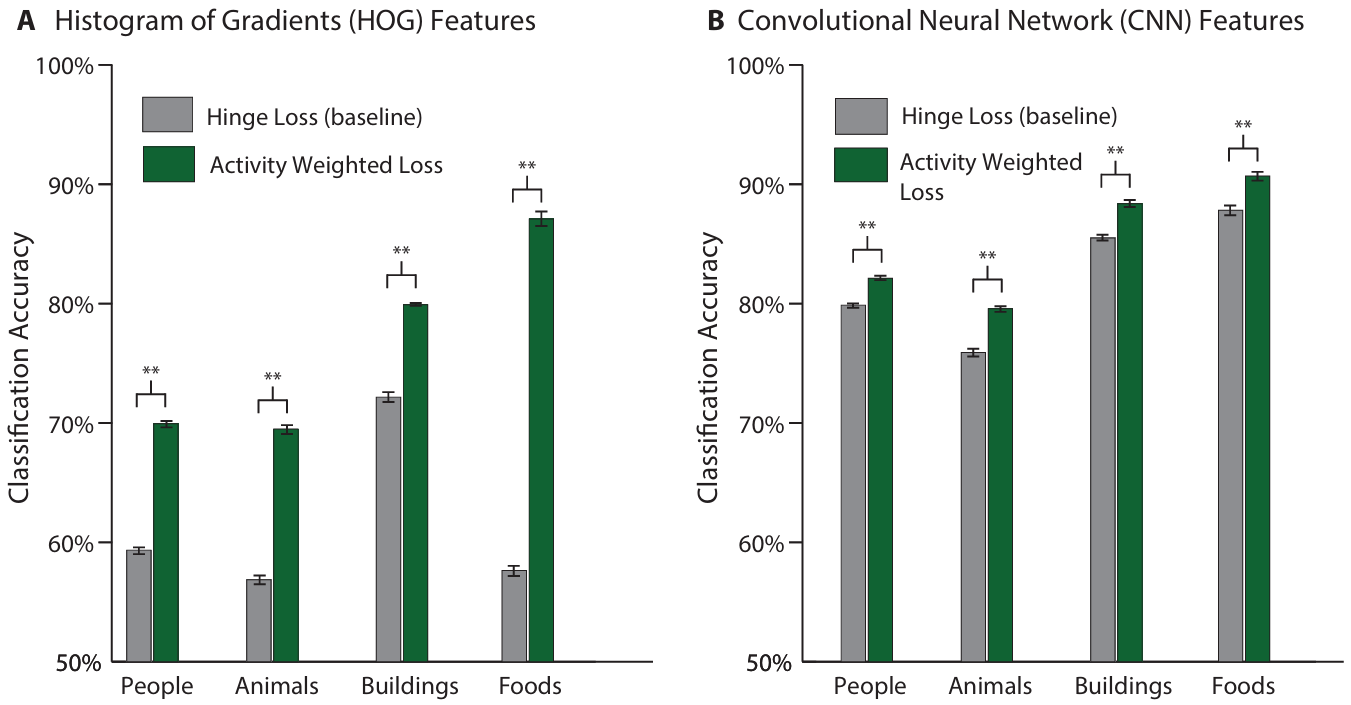
\includegraphics[width=0.65\linewidth]{images/fong.png}
    \caption{Side-by-side comparisons of the mean classification accuracy between models that were trained using either \textbf{(A)} HOG features or \textbf{(B)} CNN features and either a hinge loss (HL) or activity weighted loss (AWL) function.}
    \label{fig:fong}
\end{figure}

They also experiment using information from one brain area only for the loss, observing how this affects classification. Figure \ref{fig:fong_2} shows that certain areas produce significantly better accuracy for the specific categories they are selective for.\\

\begin{figure}[!ht]
    \centering
    \captionsetup{width=.8\linewidth}
    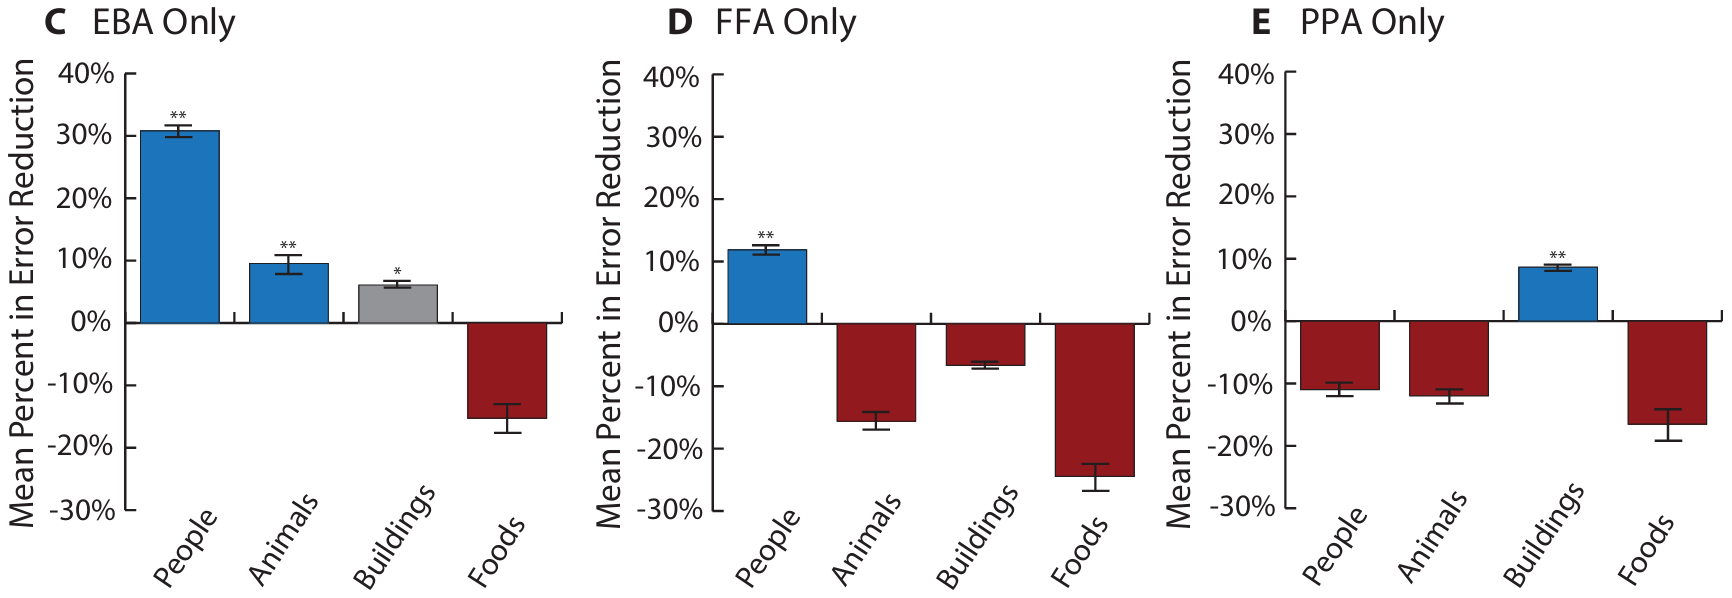
\includegraphics[width=0.7\linewidth]{images/fong_2.png}
    \caption{Mean error reductions gained by switching from HL to AWL loss when using conditioning classifies on brain activity from individual ROIs (i.e., EBA, FFA, or PPA).}
    \label{fig:fong_2}
\end{figure}

In conclusion, \textbf{information measured directly from brain can guide an ML algorithm to make better human-like decisions}.
One can harness measures of the internal representations employed by the brain to guide machine learning.
However, the authors ignore an important question: Are the better results obtained thanks to \textbf{brain} data, or is it just because it is \textbf{more} data? What if we improved the HOG classifier using AWL from CNN classifier (i.e., what if we compute the $C_x$ of the hinge loss from the CNN embeddings?).
The accuracy should be much higher, so we expect the difference when using Activity Weighted Loss to be less significant.

\section[Interpretable Semantic Vectors from a Joint Model of Brain- and Text-Based Meaning]{\textit{Interpretable Semantic Vectors from a Joint Model of Brain- and Text-Based Meaning}\\ \mandatory{fyshe-etal-2014-interpretable}}

This study is similar to \cite{fong2017using}, but the domain is completely different: human-constraint NLP. They are computational linguists and want to improve word embeddings (they are not really interested in studying the brain).

\subsection{Background}
Vector Space Models (VSMs) represent lexical meaning by assigning each word a point in high dimensional space. The high dimensional space can be any vectorial representation associated with each word. VSMs are typically created using a large text corpora. When this is he case, the VSM represents word semantics as observed in text. In the VSM, the distance between any two words is taken to indicate their semantic similarity (matching, e.g., that observed and rated by speakers). Corpus-based VSMs have been criticized as being noisy or incomplete representations of meaning.\\

When a person is reading or writing, the semantic content of each word necessarily produces patterns of activity over neurons/voxels/sensors. In principle then, \textbf{brain activity could be used instead of corpus data to construct a VSM}. If brain activation data encodes semantics, including brain data in a model of semantics could result in a more effective model. They anticipate that, if it is indeed possible to create word embeddings using brain activations, then the inclusion of this data will only improve a text-based model if brain data contains semantic information not readily available in the corpus.\\

This study tries to:
\begin{itemize}
    \item create a database of human-annotated word semantics and create a brain-informed VSM that better predicts this database,
    \item predict corpus representations of withheld words more accurately by infusing brain data into the learning model,
    \item map semantic concepts onto the brain by jointly learning neural representations.
\end{itemize}

\subsection{Data and method}
The corpus data are compiled from a 16 billion word subset of ClueWeb09 and contain two types of corpus features: \textbf{dependency} (between words) and \textbf{document features}. Dependency statistics were derived by dependency parsing the corpus and compiling co-occurence counts for all dependencies incident on the word. Count thresholding was applied to reduce noise, and positive pointwise mutual-information (PPMI \notet) was applied to the counts. SVD was applied to the document. They started with a word-by-word co-occurence matrix and then get a word-by-feature matrix $X$, after PPMI and SVD.
\osst{They consider just the positive PMI, i.e., words that co-occur more often that if they were independent.}

The brain data comes from fMRI data and MEG data for 18 subjects (9 in each imaging modality). Each read 60 concrete nouns. The 60 words span 12 word categories.\\

They adopt two methods: NNSE and JNNSE.

\subsubsection{Non-Negative Sparse Embedding (NNSE)}
They want to approximate $X$ by matrix factorization, i.e., get two matrices $A$ and $D$ that when multiplied together approximate $X$. $A$ has the same number of rows (words) as $X$, but with a much lower number of latent dimensions (they are trying to compress the feature space), $D$ instead has the same number of columns but less rows. NNSE is therefore defined as follows:
\[
\argmin_{A,D} \sum_{i=1}^w \lVert X_{i,:} - A_{i,:} \times D \rVert^2 + \lambda \lVert A\rVert_1
\]
subject to:
\[
D_{i,:}D_{i,:}^T \leq 1 \:\:\:(\forall \;1 \leq i \leq l)
\]
\[
A_{i,j} \geq 0,\:\:\: 1 \leq i \leq w,\:\:\: 1 \leq j \leq l
\]
The matrix $A$ is the output of the algorithm, i.e., the sparse approximated representation we look for (note the $\lambda \lVert A\rVert_1$ term that induces sparsity).\\

Applying NNSE is important for interpretability: without reducing the number of dimensions, the matrix is likely to have many columns that are correlated. With fewer columns, they can study them as they are not linearly dependent.
The meaning of a word is captured by finding the top-scoring dimensions for the word (i.e., the colums with highest values for the word’s row), and then finding the words that score highest on those dimensions. Each of these dimension, with the set of associated words, captures a meaning of the original word. For example, the word \textit{chair} has the following top-scoring dimensions: 
\begin{enumerate}
    \item chairs, seating, couches;
    \item mattress, futon, mattresses;
    \item supervisor, coordinator, advisor.
\end{enumerate}
These dimensions cover two of the distinct meanings of the word chair (\textit{furniture} and \textit{person of power}).

\subsubsection{Joint Non-Negative Sparse Embedding (JNNSE)}
They extend NNSEs to incorporate an additional source of data for a subset of the words in $X$, and call the approach JNNSEs.
Such algorithm allows to have a ``shared semantic space" (the matrix $A$ is an approximation of both $X$ and $Y$, $Y$ being the $word \times voxel$ matrix), and is defined as follows:
\[
\argmin_{A,D^{(c)},D^{(b)}} \sum_{i=1}^w \lVert X_{i,:} - A_{i,:} \times D^{(c)} \rVert^2 +  \sum_{i=1}^{w'} \lVert Y_{i,:} - A_{i,:} \times D^{(b)} \rVert^2 + \lambda \lVert A\rVert_1
\]
subject to:
\[
D_{i,:}^{(c)}D_{i,:}^{(c)T} \leq 1 \:\:\:(\forall \;1 \leq i \leq l)
\]
\[
D_{i,:}^{(b)}D_{i,:}^{(b)T} \leq 1 \:\:\:(\forall \;1 \leq i \leq l)
\]
\[
A_{i,j} \geq 0,\:\:\: 1 \leq i \leq w,\:\:\: 1 \leq j \leq l
\]
Notice the difference in summation. The first expression goes over all the words in the corpus ($w$), while the second goes over the subset for which we have brain data ($w'$).
$A'$ is the subset of the $A$ matrix that is relevant for reconstructing $Y$ (it is a subset of the rows in X).
Both $X$ and $Y$ can be reconstructed by multiplying $A$ with $D^{(c)}$ and $D^{(b)}$ respectively.\\

JNNSE has many advantages:
\begin{itemize}
    \item Handle partially paired data, compared to Canonical Correlation Analysis or Partial Least Squares that require data about the same observations in both cases;
    \item No need to have a common average brain (can concatenate activation across subjects in the Y matrix, per word);
    \item Merge different brain imaging experiments adding a specific loss.
\end{itemize}

\subsection{Experiments and results}
To check whether the word-by-feature matrix encodes for specific properties, they use a \textbf{probing classifier}: they train the regression model on $A$ and evaluate it on a human-rated-property table. More specifically, they obtain behavioral measure of semantics for 60 words, rated on 218 properties (e.g. \textit{smell}, \textit{emotion}, etc.), and then train the classifier to predict the [$60 \times 218$] human behavior's matrix from the $A$ matrix obtained using NNSE (text only) or JNNSE (brain+text). They experiment with different numbers of latent dimensions $l$: 250, 500 or 1000. For \textbf{evaluating the correlation} of the latent representation ($A$) with behavioral data ($Y$), they do not compare the tables directly, but use in-matrix pairwise (Euclidean) distance instead, i.e., they are somehow checking if the two vector spaces are isomorphic.\\
Figure \ref{fig:jnnse} shows that joint embeddings improve prediction of human similarity space. However, as in \cite{fong2017using}, the higher performance might not be caused by infusing brain data, but just by using a multiple data sources, which allow to remove noise.\\

Another experiment they deal with consists in \textbf{word prediction from brain data}. The matrix $A$ from NNSE or JNNSE is used as outcome variable: they predict it (for left out words) one column at a time. For each lower-dimension, there is a set of values over words ($Y$).
Regression is used to predict the value of that dimension $l$ over the $Y$ words. This is repeated for all $l$ dimensions, which produces a predictive $l$-dimensional vector per word. They train the regression on $A$ (NNSE or JNNSE) consisting of 58 words. They then produce predictive vectors for the 2 left out words and evaluate their similarity to the ground truth of those embeddings in $A$.\\
The results presented in Figure \ref{fig:jnnse_2} show how word prediction from brain data improves when the embedding space itself ($A$) is constrained by brain data.

\begin{figure}[!ht]
    \centering
    \captionsetup{width=.8\linewidth}
    \begin{subfigure}{.49\textwidth}
        \centering
        \captionsetup{width=.8\linewidth}
        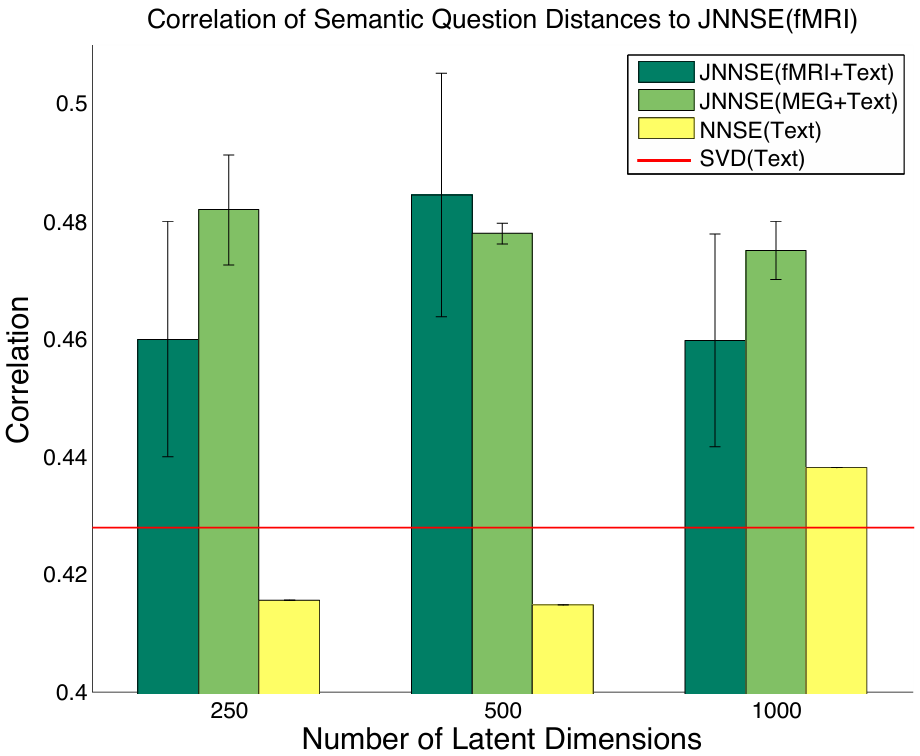
\includegraphics[width=.7\linewidth]{images/jnnse.png}
        \caption{Correlation of NNSE and JNNSE models with the distances in a semantic space constructed from behavioral data.}
        \label{fig:jnnse}
    \end{subfigure}
    \begin{subfigure}{.49\textwidth}
        \centering
        \captionsetup{width=.8\linewidth}
        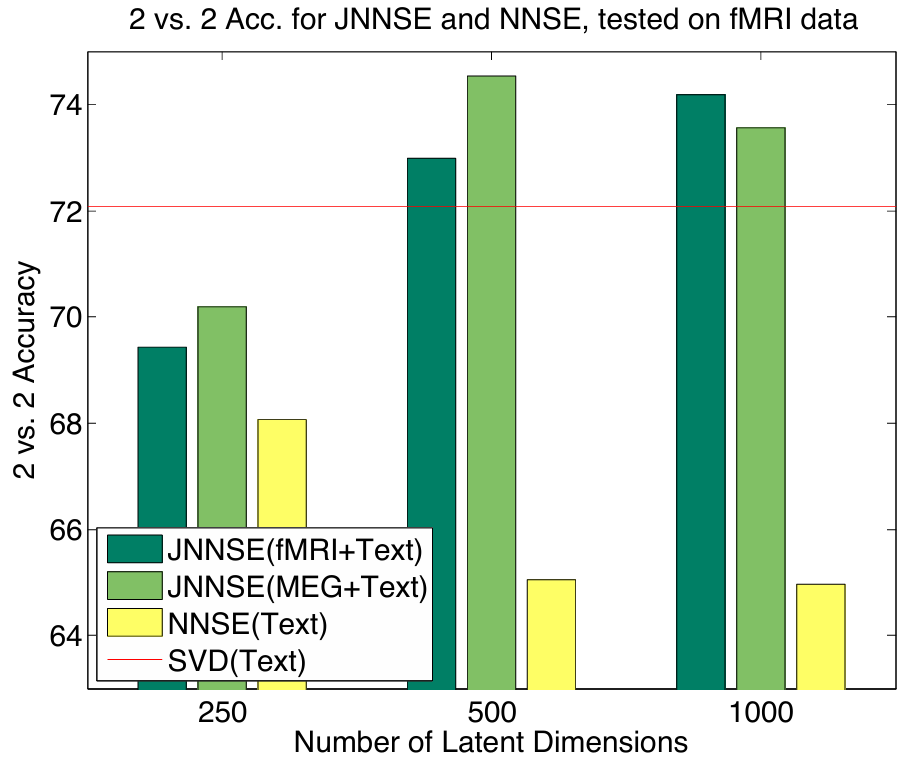
\includegraphics[width=.65\linewidth]{images/jnnse_2.png}
        \caption{Average 2~vs.~2 accuracy for NNSE and JNNSE, tested on fMRI data. Models created with one subject’s fMRI data were not used to compute 2~vs.~2 accuracy for that same subject.}
        \label{fig:jnnse_2}
    \end{subfigure}
    \caption{Comparison between NNSE and JNNSE.}
    \label{fig:jnnse_comp}
\end{figure}

Here they ask: can an accurate latent representation of a word be constructed using only brain activation data? They try to produce $X$-matrix (``raw") entries for words for which there is not enough corpus data required for creation of corpus statistics (i.e., they present rare words to people to get fMRI/MEG data). This experiment practically consists in \textbf{predicting corpus data}. They use JNNSE to obtain $A$-entries for words appearing in $X$ and $Y$ (corpus and brain), but also some words appearing only in $Y$ (brain). Notice that JNNSE allows to have brain activation entries without the corresponding corpus entries.
Then, $D^{(c)}$ in used to recreate the entries for those words.\\
They compute a rank accuracy measure and the mean rank accuracy is as high as 67\% for $l=500$.\\

The last experiment consists in \textbf{mapping semantics onto the brain}. $D^{(b)}$ is a [$l \times v$] matrix (\textit{latent dimensions} $\times$ \textit{voxels}). This allows to obtain a brain map for each dimension $l$ in that matrix. They tweak the importance of the perceptual features ($Y$) by scaling their values (details missing; but we can consider weighting schemes). They plot these dimensions on brain slices. They can find a brain area, link it to the dimension that predicted it, and see which words load strongly on that dimension. This allows to study how different groups (age, culture, etc.) have different representations of language.

\begin{wrapfigure}[12]{r}{0pt}
  \centering
  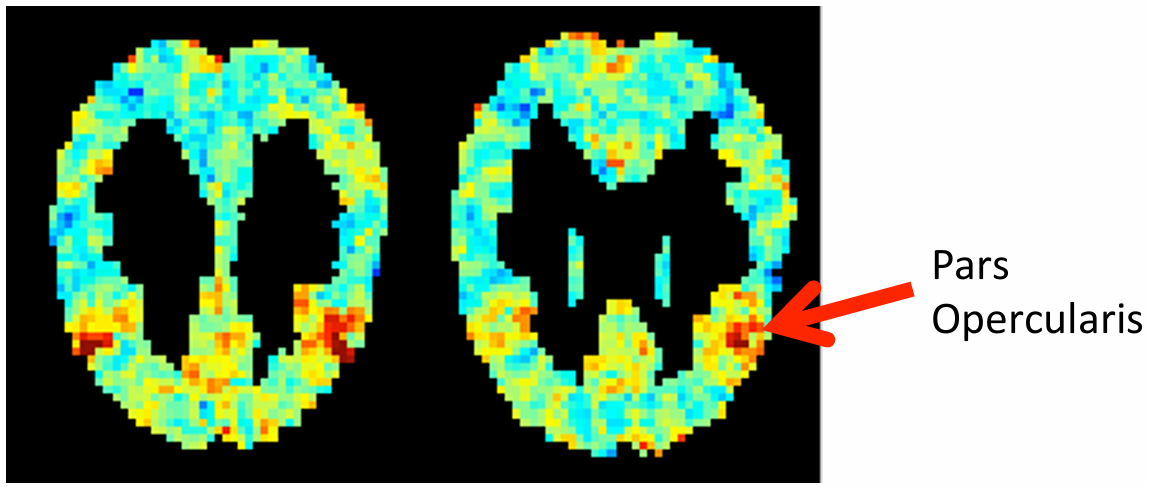
\includegraphics[width=0.4\textwidth]{images/jnnse_4.png}
  \caption{$D^{(b)}$ matrix; dimension with top scoring words \textit{buffet}, \textit{brunch}, \textit{lunch}. Pars opercularis is believed to be part of the gustatory cortex, which responds to food related words.}
  \label{fig:jnnse_4}
\end{wrapfigure}
In Figure \ref{fig:jnnse_4} there is an example (through fMRI slices) of mapping ($D^{(b)}$) from latent semantic space ($A$) to brain space ($Y$) for fMRI and words from three semantic categories.\\

In conclusion, VSMs can be extended or even substituted using brain data. Addition of brain data strongly improves the prediction of human annotations (perhaps can substitute them) and the prediction of latent dimension scores produced in the joint embedding. It is possible to use brain data to synthesize raw corpus data for those words. And finally, solutions of joint embeddings can be mapped onto the brain space.

